\section{The Vanishing Gradient Problem}

\definecolor{darkgreen}{rgb}{0,0.6,0}


% -----------------------------------------------------------------------------
\mode<article>{
    \begin{figure}[h]
        \centering
        \includegraphics[height=1cm]{img/simple_arch_color}
         \caption{A simple network with a chain of neurons.}
         \label{fig:chain}
    \end{figure}
}
\begin{frame}\frametitle{\secname}
\mode<presentation>{
	\begin{center}
		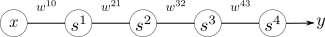
\includegraphics[width=10cm]{img/simple_arch}
	\end{center}
	}
	Compute $\frac{\partial y}{\partial w^{10}}\ldots$
	
	\begin{enumerate}
	\item via the chain rule
	\item using the Backpropagation algorithm
	\end{enumerate}
\end{frame}
% -----------------------------------------------------------------------------
\begin{frame}\frametitle{\secname}
\mode<presentation>{
	\begin{center}
		\includegraphics[width=10cm]{img/simple_arch_color}
	\end{center}
	}
    forward pass:
    \slidesonly{
    \vspace{-5mm}
    }
	\begin{equation}
            {h_i^{v'}} 
            := 
            \only<+->{
            \kern-2ex
            \sum_{(\mu,k) \in P(v',\,i)}
            \kern-2ex
            w_{ik}^{v'\mu}\cdot
            f_k^\mu\big( {h_k^\mu} \big) 
            }
            \only<+->{
            \stackrel{{
    \substack{\text{this}\\ \text{model}}}
    }{=} w^{v'v}\cdot
            f\big( {h^{v}} \big)   
            }
    \end{equation}
    
    where $v=v'-1$
    \slidesonly{
    \vspace{-5mm}
    }
    
    \begin{align}
    y\;\;&=\;\;
    \only<+->{
    {\color{blue}s^4} = {\color{blue}f(h^{4})}\\
    }
    \only<+->{
    \;\;&=\;\;
    {\color{blue}
    f\big({\color{black}w^{43} \cdot} {\color{magenta}f(h^{3})}\big)
    }\\
    }
    \only<+->{
    \;\;&=\;\;
    {\color{blue}
    f\Big({\color{black}w^{43} \cdot} {\color{magenta}f\big({\color{black}w^{32} \cdot} {\color{darkgreen}f(h^{2})}\big)}\Big)
    }\\
    }
    \only<+->{
    \;\;&=\;\;
    {\color{blue}
    f\Big({\color{black}w^{43} \cdot }{\color{magenta}f\Big({\color{black}w^{32} \cdot} {\color{darkgreen}f\big({\color{black}w^{21} \cdot} {\color{red}f(h^{1})}\big)}\Big)}\Big)
    }\\
    }
    \only<+->{
    \;\;&=\;\;
    {\color{blue}
    f\Big({\color{black}w^{43} \cdot } {\color{magenta}f\Big({\color{black}w^{32} \cdot} {\color{darkgreen}f\big({\color{black}w^{21} \cdot} {\color{red}f({\color{black}w^{10} \cdot x})}\big)}\Big)}\Big)
    }
    }
    \end{align}
\end{frame}

% -----------------------------------------------------------------------------
\begin{frame}\frametitle{\secname}
\mode<presentation>{
	\begin{center}
		\includegraphics[width=10cm]{img/simple_arch_color}
	\end{center}
	}
    backward pass:
    \begin{align}
     \frac{\partial y}{\partial w^{10}}
     \;\;&\stackrel{\mathclap{
    \substack{\text{chain}\\ \text{rule}}}
    }{=}\;\;
    \only<+->{
    \frac{\partial y}{\partial h^{\color{red}1}}
    \cdot \frac{\partial h^{\color{red}1}}{\partial w^{10}}\\
    }
    \only<+->{
    \;\;&=\;\;
    \frac{\partial y}{\partial h^{\color{darkgreen}2}}
    \cdot \frac{\partial h^{\color{darkgreen}2}}{\partial h^{\color{red}1}}
    \cdot \frac{\partial h^{\color{red}1}}{\partial w^{10}}\\
    }
    \only<+->{
    \;\;&=\;\;
    \frac{\partial y}{\partial h^{\color{magenta}3}}
    \cdot \frac{\partial h^{\color{magenta}3}}{\partial h^{\color{darkgreen}2}}
    \cdot \frac{\partial h^{\color{darkgreen}2}}{\partial h^{\color{red}1}}
    \cdot \frac{\partial h^{\color{red}1}}{\partial w^{10}}\\
    }
    \only<+->{
    \;\;&=\;\;
    \frac{\partial y}{\partial h^{\color{blue}4}}
    \cdot \frac{\partial h^{\color{blue}4}}{\partial h^{\color{magenta}3}}
    \cdot \frac{\partial h^{\color{magenta}3}}{\partial h^{\color{darkgreen}2}}
    \cdot \frac{\partial h^{\color{darkgreen}2}}{\partial h^{\color{red}1}}
    \cdot \frac{\partial h^{\color{red}1}}{\partial w^{10}}\\
    }
    \only<+->{
    \;\;&=\;\;
    f'(h^{\color{blue}4})  \cdot w^{43} f'(h^{\color{magenta}3}) \cdot w^{32}  f'(h^{\color{darkgreen}2}) \cdot  w^{21} f'(h^{\color{red}1}) \cdot x
    }
    \end{align}
\end{frame}

\subsection{Using the Backpropagation algorithm}

\begin{frame}\frametitle{\subsecname}
\mode<presentation>{
	\begin{center}
		\includegraphics[width=7cm]{img/simple_arch_color}
	\end{center}
	\vspace{-5mm}
	Recall that
	}
	    \begin{equation}
            \only<+->{
        {\delta_i^{v'}}
        =
        [f_i^{v'}]'({h_i^{v'}}) 
        \kern-3ex\sum_{(v''\hspace{-1mm},\,k) \in C(v',\,i)}\kern-3ex
        {\delta_k^{v''}} 
        {w}_{ki}^{v'' v'}
        }
            \stackrel{{
    \substack{\text{this}\\ \text{model}}}
    }{=} 
            \only<+->{
            f'({h^{v'}}) \,
        {w}^{v'' v'} \cdot
    {\delta^{v''}} 
            }
    \end{equation}
    
    and 
    \slidesonly{
	\vspace{-5mm}
	}
    
    \begin{equation}
     \frac{\partial y}{\partial w^{v'v}} = 
				{ \delta^{v'}} \kern-.5ex\cdot
			   			f^v( {h^v} )
    \end{equation}
    
    Therefore:
    \slidesonly{
	\vspace{-8mm}
	}
    
    \begin{align}
     \frac{\partial y}{\partial w^{10}} 
     &= \delta^{1} \cdot x \\
	 &= x \cdot f'(h^{\color{red}1}) w^{21} \cdot \delta^2\\
	 &= x \cdot f'(h^{\color{red}1}) w^{21} \cdot f'(h^{\color{darkgreen}2}) w^{32} \cdot \delta^3\\
	 &= x \cdot f'(h^{\color{red}1}) w^{21} \cdot f'(h^{\color{darkgreen}2}) w^{32} \cdot f'(h^{\color{magenta}3}) w^{43} \cdot \delta^4\\
	 &= x \cdot f'(h^{\color{red}1}) w^{21} \cdot f'(h^{\color{darkgreen}2}) w^{32} \cdot f'(h^{\color{magenta}3}) w^{43} \cdot f'(h^{\color{blue}4})
    \end{align}
\end{frame}
